\documentclass{article}
\usepackage{tikz}
\usepackage{amsmath}
\usepackage{bm}
\usepackage{scalerel}
\usepackage{pgfplots}
\usepackage{mathpazo}
\pgfplotsset{width=9cm,compat=1.8}
\usetikzlibrary{patterns}
\usetikzlibrary{arrows,shapes,calc}
\usetikzlibrary{external}
\tikzset{external/system call={pdflatex \tikzexternalcheckshellescape -halt-on-error
        -interaction=batchmode -jobname "\image" "\texsource" && %  or ;
pdftops -eps "\image".pdf}}
\tikzexternalize




\begin{document}
	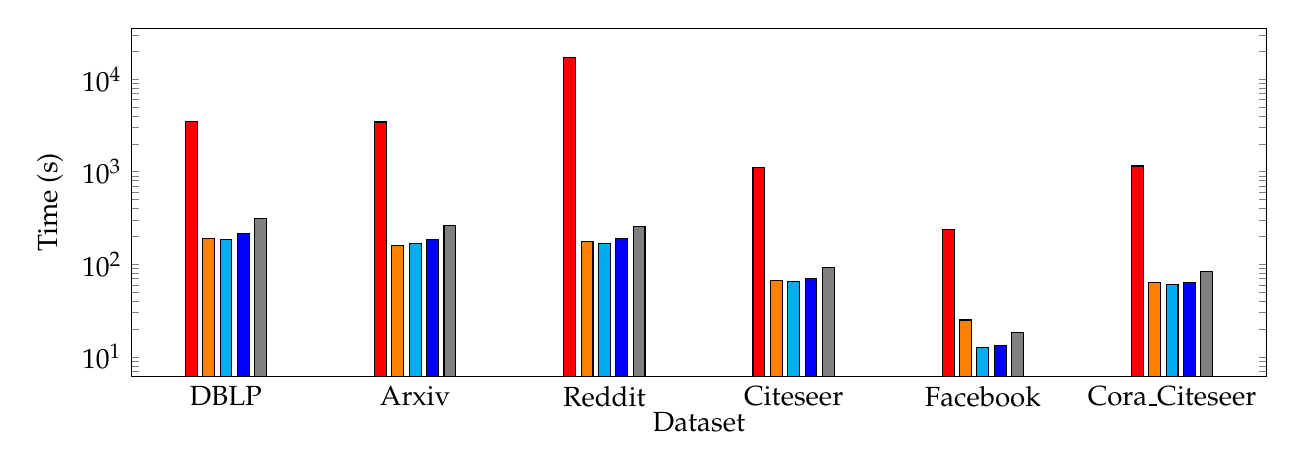
\begin{tikzpicture}
		\definecolor{lssfre}{HTML}{fccde5} %粉
		\definecolor{lssemb}{HTML}{bc80bd} %紫色
		\definecolor{lsscon}{HTML}{bebada} %淡紫色
		\definecolor{wj}{HTML}{fb8072} %橙色 深一点
		\definecolor{impr}{HTML}{80b1d3} %青蓝
		\definecolor{cs}{HTML}{fdb462} %橙色
		\definecolor{cset}{HTML}{b3de69}%绿色
		\definecolor{jsub}{HTML}{8dd3c7} %青绿
		\definecolor{sumrdf}{HTML}{ffffb3} %淡黄
		\definecolor{bsk}{HTML}{d9d9d9} %浅灰
		\definecolor{gflow}{HTML}{778899} %深灰色
		\definecolor{SB}{HTML}{F5F5DC}
		\definecolor{lc}{HTML}{FFFDD0}
		\definecolor{fire}{HTML}{FFE5B4}
		\definecolor{bo}{HTML}{E6E6FA}
		\definecolor{PINK}{HTML}{FFC0CB}
		\centering
		\begin{axis}
			%\label{fig:train time}
			[
			ybar, %axis on top,
			height=6cm, 
			width=16cm,
			bar width=0.15cm,
			tick align=inside,
			%enlarge y limits={value=.1,upper},
			%ymin=0, ymax=100000,
			tickwidth=0pt,
			ymode=log,
			log origin=infty,
			enlarge x limits=true,
			legend style={
				draw=none,
				at={(0.5, 1.3)},
				anchor=north,
				legend columns=5,
				/tikz/every even column/.append style={column sep=0.2cm}
			},
			ylabel={Time (s)},
			%ytick={1, 100, 10000},
			%yticklabels={$1$,$10^2$, $10^4$},
			xmin=3, xmax = 18,
			xtick={3,6,9,12,15,18 },
			xticklabels={DBLP ,Arxiv ,Reddit, Citeseer, Facebook, Cora\_Citeseer},
			xlabel={Dataset},
			xlabel style={yshift=1ex},
			%symbolic x coords={
			%	Arxiv, Citeseer, Cora, Facebook, Cora\_Citeseer },
			%xtick=data,
			]
			
			% MAML
			\addplot [ybar, fill=red, area legend] coordinates {
				(3, 3455.7079)
				(6, 3445.6243)
				(9, 17253.3743)
				(12, 1102.187)	
				(15, 239.7145)	
				(18, 1151.4864)
			};
			
			% FeatTrans
			\addplot [ybar, fill=orange, area legend] coordinates {
				(3, 189.8072)
				(6, 160.3456)
				(9, 175.7211)
				(12, 66.2556)	
				(15,24.9775)
				(18,63.922)
			};
			
			% CGNP
			\addplot [ybar, fill=cyan, area legend] coordinates {	
				(3, 186.7565)
				(6, 167.081)
				(9, 169.4361)
				(12, 64.8826)	
				(15, 12.7299)
				(18,60.18)
			};
			
			% CGNP_MLP
			\addplot [ybar, fill=blue, area legend] coordinates {
				(3, 212.7159)
				(6, 185.0568)
				(9, 189.9457)
				(12, 69.4228)	
				(15, 13.281)
				(18, 63.3159)
			};
			
			% CGNP_GNN
			\addplot [ybar, fill=gray, area legend] coordinates {
				(3,312.0491)
				(6, 263.5118)
				(9, 257.1656)
				(12, 91.3902)	
				(15, 18.1759)
				(18, 84.1433)
			};
			
			
			\legend{
			%	\large $\texttt{MAML}$,
			%	\large $\texttt{FeatTrans}$,
			%	\large $\texttt{CGNP}$,
			%	\large $\texttt{CGNP\_MLP}$,
			%	\large $\texttt{CGNP\_GNN}$
			}
			
		\end{axis}
	\end{tikzpicture}

\end{document}
